\documentclass{standalone}
\usepackage{tikz}
\usetikzlibrary{patterns}
\usetikzlibrary{positioning}
\usetikzlibrary{patterns, positioning}
\usetikzlibrary{shapes.misc}
\usepackage[outline]{contour}
\contourlength{1.5pt} 
\usepackage[sfdefault]{ClearSans}

\begin{document}
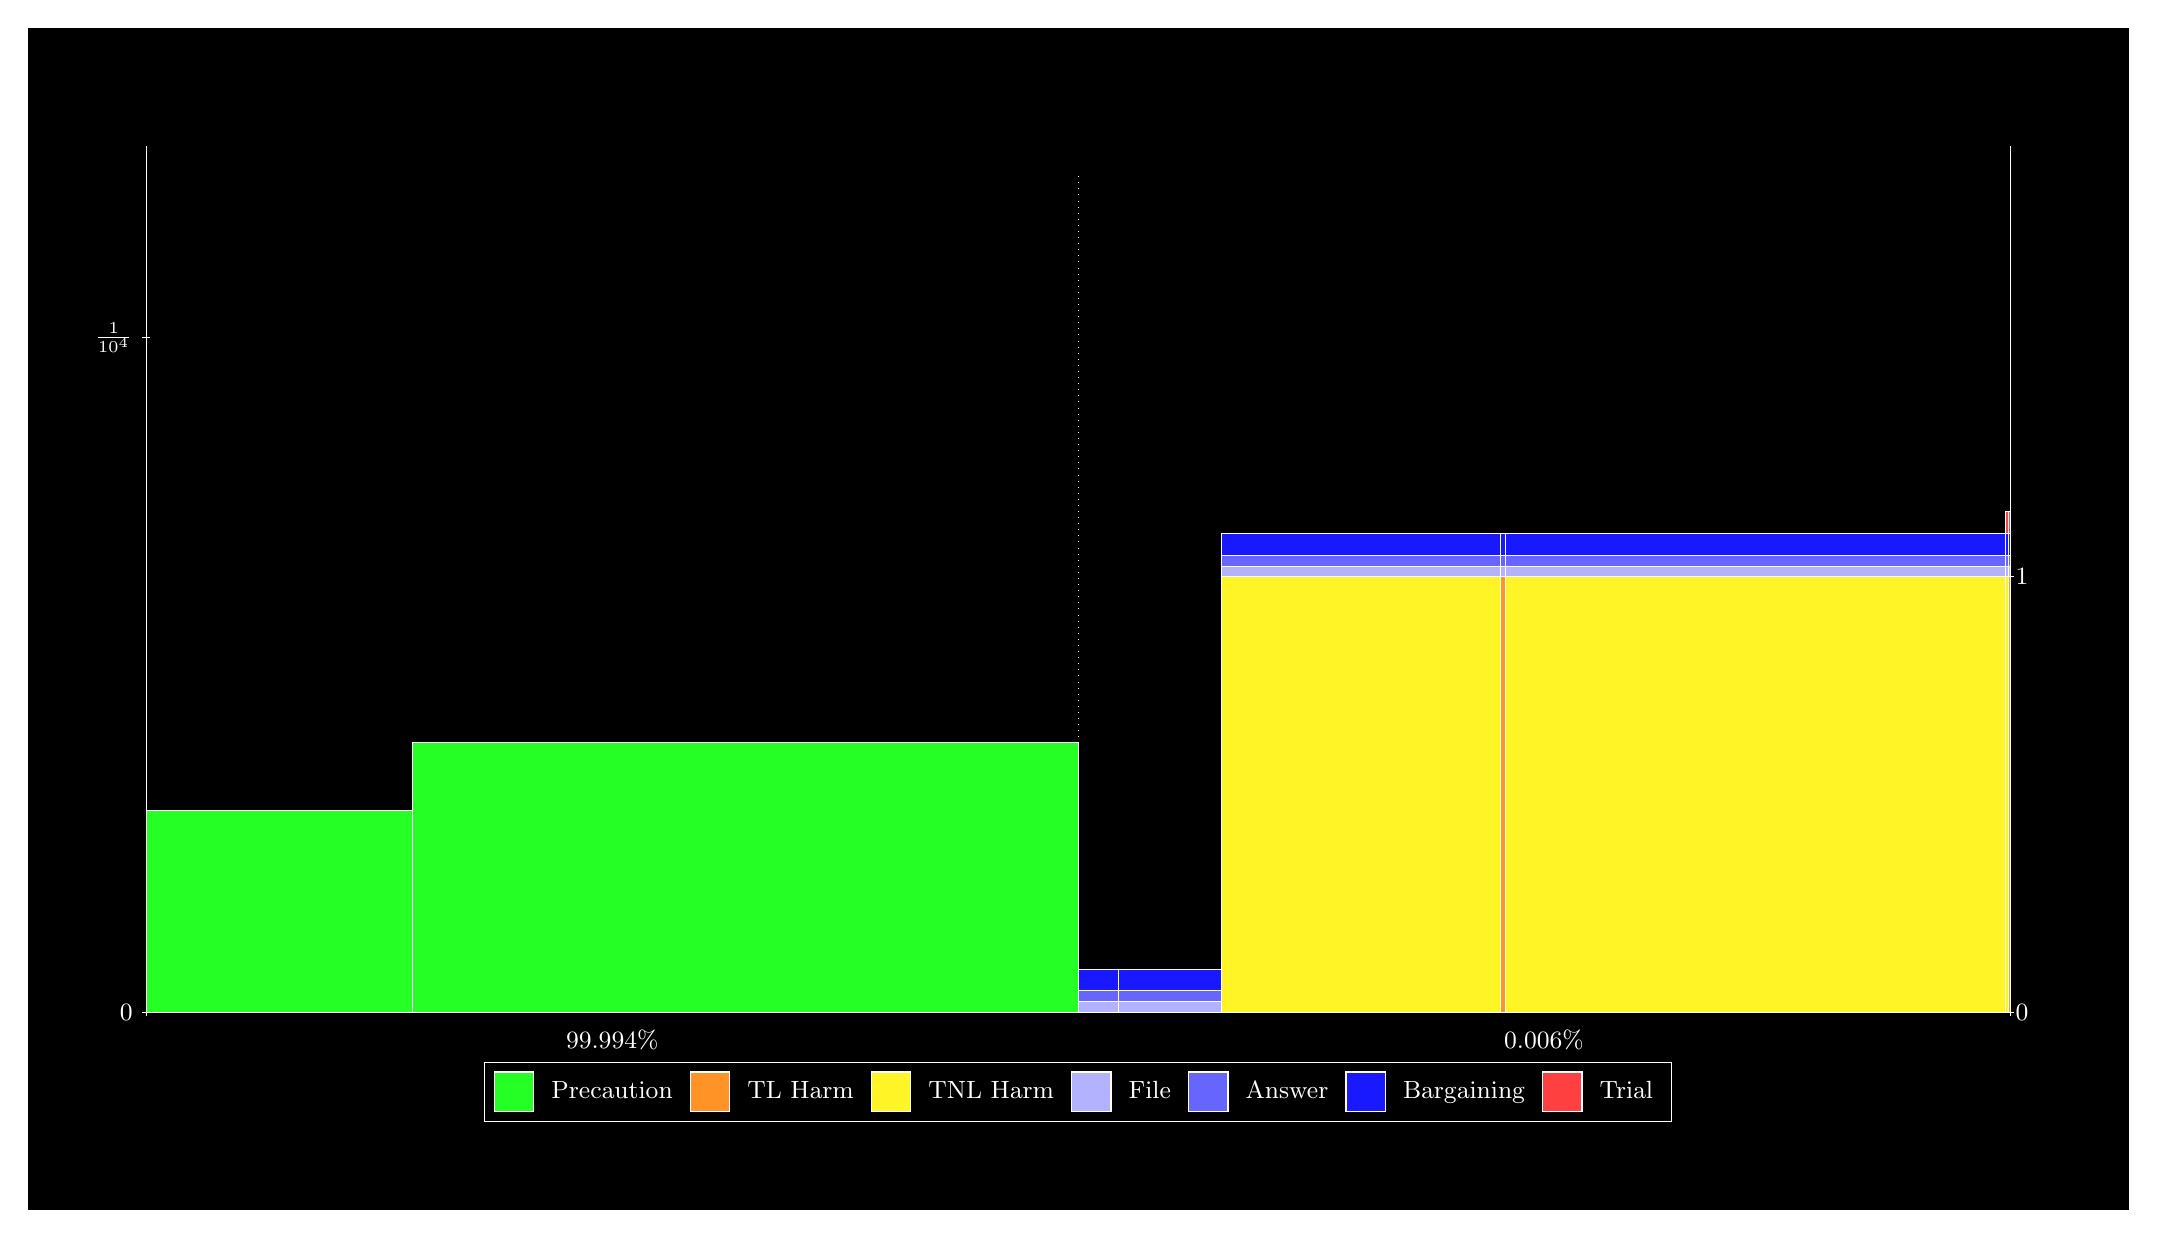
\begin{tikzpicture}
\draw[fill=black] (0,0) rectangle (26.667,15);
\draw[fill=green!85,draw=white,very thin] (1.5,2.5) rectangle (4.8736,5.0715);
\draw[fill=green!85,draw=white,very thin] (4.8736,2.5) rectangle (13.333,5.9287);
\draw[fill=green!85,draw=white,very thin] (13.333,2.5) rectangle (13.846,2.5002);
\draw[fill=blue!30,draw=white,very thin] (13.333,2.5002) rectangle (13.846,2.6385);
\draw[fill=blue!60,draw=white,very thin] (13.333,2.6385) rectangle (13.846,2.7768);
\draw[fill=blue!90,draw=white,very thin] (13.333,2.7768) rectangle (13.846,3.0535);
\draw[fill=green!85,draw=white,very thin] (13.846,2.5) rectangle (15.156,2.5002);
\draw[fill=blue!30,draw=white,very thin] (13.846,2.5002) rectangle (15.156,2.6386);
\draw[fill=blue!60,draw=white,very thin] (13.846,2.6386) rectangle (15.156,2.7769);
\draw[fill=blue!90,draw=white,very thin] (13.846,2.7769) rectangle (15.156,3.0536);
\draw[fill=green!85,draw=white,very thin] (15.156,2.5) rectangle (18.694,2.5002);
\draw[fill=yellow!85,draw=white,very thin] (15.156,2.5002) rectangle (18.694,8.0336);
\draw[fill=blue!30,draw=white,very thin] (15.156,8.0336) rectangle (18.694,8.1719);
\draw[fill=blue!60,draw=white,very thin] (15.156,8.1719) rectangle (18.694,8.3103);
\draw[fill=blue!90,draw=white,very thin] (15.156,8.3103) rectangle (18.694,8.5869);
\draw[fill=green!85,draw=white,very thin] (18.694,2.5) rectangle (18.757,2.5002);
\draw[fill=orange!85,draw=white,very thin] (18.694,2.5002) rectangle (18.757,8.0336);
\draw[fill=blue!30,draw=white,very thin] (18.694,8.0336) rectangle (18.757,8.1719);
\draw[fill=blue!60,draw=white,very thin] (18.694,8.1719) rectangle (18.757,8.3103);
\draw[fill=blue!90,draw=white,very thin] (18.694,8.3103) rectangle (18.757,8.5869);
\draw[fill=green!85,draw=white,very thin] (18.757,2.5) rectangle (25.109,2.5002);
\draw[fill=yellow!85,draw=white,very thin] (18.757,2.5002) rectangle (25.109,8.0336);
\draw[fill=blue!30,draw=white,very thin] (18.757,8.0336) rectangle (25.109,8.172);
\draw[fill=blue!60,draw=white,very thin] (18.757,8.172) rectangle (25.109,8.3103);
\draw[fill=blue!90,draw=white,very thin] (18.757,8.3103) rectangle (25.109,8.587);
\draw[fill=green!85,draw=white,very thin] (25.109,2.5) rectangle (25.14,2.5002);
\draw[fill=yellow!85,draw=white,very thin] (25.109,2.5002) rectangle (25.14,8.0336);
\draw[fill=blue!30,draw=white,very thin] (25.109,8.0336) rectangle (25.14,8.1719);
\draw[fill=blue!60,draw=white,very thin] (25.109,8.1719) rectangle (25.14,8.3103);
\draw[fill=blue!90,draw=white,very thin] (25.109,8.3103) rectangle (25.14,8.5869);
\draw[fill=red!75,draw=white,very thin] (25.109,8.5869) rectangle (25.14,8.8636);
\draw[fill=green!85,draw=white,very thin] (25.14,2.5) rectangle (25.167,2.5002);
\draw[fill=orange!85,draw=white,very thin] (25.14,2.5002) rectangle (25.167,8.0336);
\draw[fill=blue!30,draw=white,very thin] (25.14,8.0336) rectangle (25.167,8.1719);
\draw[fill=blue!60,draw=white,very thin] (25.14,8.1719) rectangle (25.167,8.3103);
\draw[fill=blue!90,draw=white,very thin] (25.14,8.3103) rectangle (25.167,8.5869);
\draw[fill=red!75,draw=white,very thin] (25.14,8.5869) rectangle (25.167,8.8636);
\draw[white,very thin] (1.5,2.5) -- (1.5,13.5);
\draw[white,very thin] (1.45,2.5) -- (1.55,2.5);
\node[font=\small,text=white, anchor=east] at (1.45, 2.5) {0};
\draw[white,very thin] (1.45,11.072) -- (1.55,11.072);
\node[font=\small,text=white, anchor=east] at (1.45, 11.072) {$\frac{1}{10^{4}}$};

\draw[white,dotted,very thin] (13.333,2.83) -- (13.333,13.17);
\draw[white,very thin] (25.167,2.5) -- (25.167,13.5);
\draw[white,very thin] (25.117,2.5) -- (25.217,2.5);
\node[font=\small,text=white, anchor=west] at (25.117, 2.5) {0};
\draw[white,very thin] (25.117,8.0334) -- (25.217,8.0334);
\node[font=\small,text=white, anchor=west] at (25.117, 8.0334) {1};

\draw[white,very thin] (1.5,2.5) -- (25.167,2.5);
\draw[white,very thin] (1.5,2.45) -- (1.5,2.55);
\node[font=\small,text=white, anchor=north] at (1.5, 2.45) {};
\draw[white,very thin] (25.167,2.45) -- (25.167,2.55);
\node[font=\small,text=white, anchor=north] at (25.167, 2.45) {};

\node[font=\small,text=white,anchor=south] at (7.4167, 1.9) {99.994\%};
\node[font=\small,text=white,anchor=south] at (19.25, 1.9) {0.006\%};
\draw (13.3333,2.5) node (B) {};
\begin{scope}[align=center]
\matrix[scale=0.5,draw=white,below=0.5cm of B,nodes={draw},column sep=0.1cm]{
\node[rectangle,draw,minimum width=0.5cm,minimum height=0.5cm,fill=green!85]{}; & \node[draw=none,font=\small,text=white]{Precaution}; &
\node[rectangle,draw,minimum width=0.5cm,minimum height=0.5cm,fill=orange!85]{}; & \node[draw=none,font=\small,text=white]{TL Harm}; &
\node[rectangle,draw,minimum width=0.5cm,minimum height=0.5cm,fill=yellow!85]{}; & \node[draw=none,font=\small,text=white]{TNL Harm}; &
\node[rectangle,draw,minimum width=0.5cm,minimum height=0.5cm,fill=blue!30]{}; & \node[draw=none,font=\small,text=white]{File}; &
\node[rectangle,draw,minimum width=0.5cm,minimum height=0.5cm,fill=blue!60]{}; & \node[draw=none,font=\small,text=white]{Answer}; &
\node[rectangle,draw,minimum width=0.5cm,minimum height=0.5cm,fill=blue!90]{}; & \node[draw=none,font=\small,text=white]{Bargaining}; &
\node[rectangle,draw,minimum width=0.5cm,minimum height=0.5cm,fill=red!75]{}; & \node[draw=none,font=\small,text=white]{Trial}; \\\\
};\end{scope}

\end{tikzpicture}
\end{document}